\documentclass[xcolor=dvipsnames]{beamer}
\usepackage{caption}

\renewcommand{\thefootnote}{\arabic{footnote}}

\usetheme{Madrid}
\useoutertheme{miniframes} % Alternatively: miniframes, infolines, split
\useinnertheme{circles}

\setbeamerfont{frametitle}{size=\footnotesize}

\setbeamercolor{section in toc}{fg=black,bg=black}
\setbeamercolor{alerted text}{fg=black}
\setbeamercolor*{palette primary}{fg=white,bg=gray} % cadre autour du titre + rectangle bas droite.
\setbeamercolor*{palette secondary}{fg=yellow,bg=yellow}
\setbeamercolor*{palette tertiary}{bg=black,fg=gray!10!white} % carré du milieu + bande en header. 
\setbeamercolor*{palette quaternary}{fg=yellow,bg=yellow}
\setbeamercolor*{sidebar}{fg=black,bg=gray!15!white}
%\setbeamercolor*{titlelike}{parent=palette primary}
\setbeamercolor{titlelike}{parent=palette primary,fg=black}
\setbeamercolor{frametitle}{bg=white}
\setbeamercolor{frametitle right}{bg=gray!60!white}
\setbeamercolor*{separation line}{}
\setbeamercolor*{fine separation line}{}
% Override palette coloring with secondary
\setbeamercolor{subsection in head/foot}{bg=gray,fg=white}
\setbeamercolor{local structure}{fg=black} % changer la couleur des enumerate et itemize.
\setbeamertemplate{caption}[numbered]
\title[Analyse d'articles scientifiques avec R]{Analyse textuelle d’articles scientifiques évaluant l’impact des vers de terre sur l’environnement}
\subtitle{Une approche \textit{tidy} pour l'analyse textuelle d'articles scientifiques avec 
\includegraphics[scale=0.04]{R_logo.svg.png}}
\author[Stage M1 BIMS]{Antoine MALET - Stage M1, Parcours BIMS}
\institute[UMR MIA Paris-Saclay]{Campus Agro Paris-Saclay - Unité Mathématiques et Informatique Appliqués}
\date{03/07/2024}

\begin{document}

\setbeamertemplate{headline}{}

	\begin{frame}
		\titlepage
	\end{frame}
	
\setbeamertemplate{headline}[miniframes theme]

	\section*{Introduction}
	\subsection*{Contexte scientifique / Objectifs} % PBTQ, à remettre dans chaque ss.

	\begin{frame}
		\frametitle{\underline{Contexte scientifique:}}
		\textbf{Rôle écologique du vers de terre: deux contextes géographiques qui s'opposent dans la littérature scientifique.}
		\begin{columns}
			\begin{column}{0.5\textwidth} % permet diviser la frame en deux colonnes, chacune occupant 50% de l'espace total disponible.
				\begin{enumerate}
					\item Europe : Importantes fonctions économiques et écosystémiques (productivité/richesse des sols).
					\vspace{\baselineskip}
					\item Amérique du nord : Espèce invasive = dommages écosystémiques importants.
					% (altération des sols / perturbation de la biodiversité chez les espèces natives)
				\end{enumerate}
			\end{column}
			\begin{column}{0.5\textwidth}
				\begin{figure}[htb] %le h entre crochet signifie je veux la figure à cet emplacement
					\begin{center} %centrer la figure
						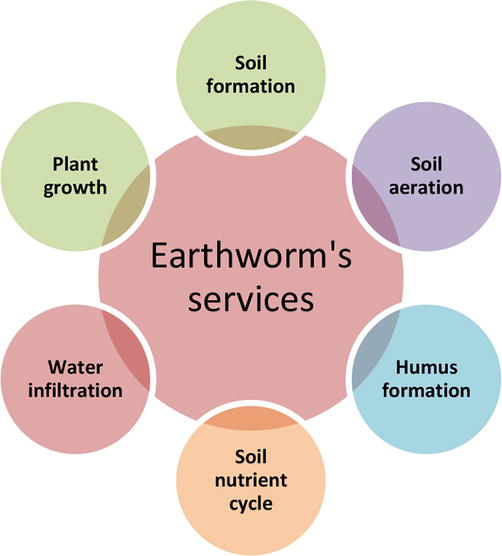
\includegraphics[width=0.4\textwidth]{EW_services.png}
						\caption{Les services écosystémiques rendus par les vers de terre\footnotemark.}\label{fig_wormsservices}
						%legende
					\end{center}
				\end{figure}
			\end{column}
		\end{columns}
		\footnotetext{\textit{Extrait de:} The Earthworms: Charles Darwin’s Ecosystem Engineer, Kumar et al.  (2023).}
	\end{frame}

	\begin{frame}
		\frametitle{\underline{Objectifs:}}
		\textbf{Les méthodes informatiques et statistiques de} \textit{Web-scraping} \textbf{et de} \textit{Text-mining} \textbf{permettent-elles de mettre en évidence cette opposition grâce à une approche automatisable ?}
		
		\vspace{\baselineskip}
		\begin{enumerate}
				\item \textbf{Données:} Données textuelles (vers de terre), 4 métaanalyses et leur corpus\footnote{
					1.“Soil chemistry turned upside down: a meta-analysis of invasive earthworm effects on soil chemical properties”
					2.“Earthworms affect plant growth and resistance against herbivores: A meta-analysis”
					3.“The unseen invaders: introduced earthworms as drivers of change in plant communities in North American forests (a meta-analysis)”
					4.“Earthworms increase plant production: a meta-analysis”} (\textit{deux positives et deux négatives}).
				\item \textbf{Objectif:} Tenter de retrouver cette opposition grâce à des méthodes statistiques automatisables.
				\item \textbf{Méthodes:} \textit{Web scraping} avec Python / \textit{Text-mining} avec R.
			\end{enumerate}
	\end{frame}

	\section*{Données et scripts}
	\subsection*{Base de données / Scripts} % PBTQ, à remettre dans chaque ss.
	\begin{frame}
		\frametitle{\underline{Base de données:}}
		\begin{columns}
			\begin{column}{0.4\textwidth} % permet diviser la frame en deux colonnes, chacune occupant 50% de l'espace total disponible.
				\begin{enumerate}
					\item Ligne: 1 article / ligne.
					\item La colonne "Abstract" est la plus importante, car elle contient les \textit{textes à analyser}.
				\end{enumerate}
			\end{column}
			\begin{column}{0.6\textwidth}
				\begin{figure}[htb] %le h entre crochet signifie je veux la figure à cet emplacement
					\begin{center} %centrer la figure
						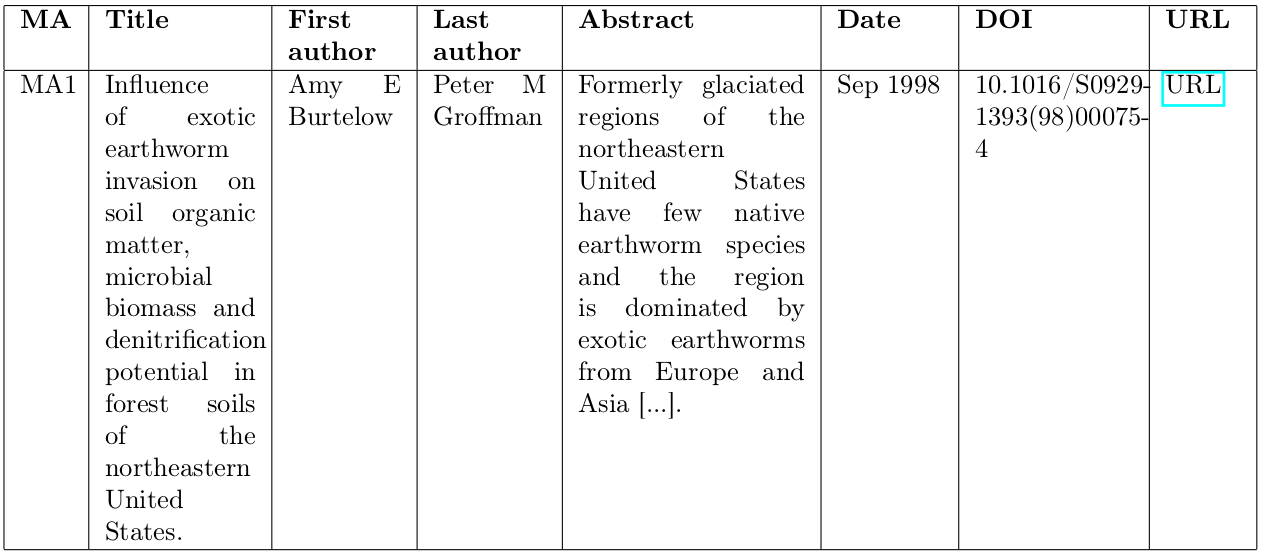
\includegraphics[width=1\textwidth]{screenshotCSV.png}
						\caption{Tableau présentant un exemple de la structure type du fichier CSV issu du Web-scraping et
						employé pour l’analyse. Le fichier originel comprend 168 lignes. Les données manquantes (non représentées ici), sont
						notées "N/A".}\label{fig_exemple_bdd}
						%legende
					\end{center}
				\end{figure}
			\end{column}
		\end{columns}
	\end{frame}

	\begin{frame}
		\frametitle{\underline{Scripts Python et R:}}
		\begin{columns}
			\begin{column}{0.5\textwidth} % permet diviser la frame en deux colonnes, chacune occupant 50% de l'espace total disponible.
				\begin{enumerate}
					\item \textbf{Script Python:} Pour le Web-scraping. \\ \textit{Principaux modules: habanero (Crossref) / ittertools / numpy / pandas / unidecode / ResearchGateScraper2 (module local, incluant re, time, parsel et playwright.sync\_api)}.
					\item \textbf{Script R:} Pour le Text-mining. \\ \textit{Principaux modules: dplyr, ggplot2, ggraph, SnowballC, scales, tidytext.}
				\end{enumerate}
			\end{column}
			\begin{column}{0.5\textwidth}
				\begin{figure}[htb] %le h entre crochet signifie je veux la figure à cet emplacement
					\begin{center} %centrer la figure
						
\includegraphics[width=0.5\textwidth]{image_python_R.png}
						\caption{Le code de Web-scraping a été implémenté en Python, le code de Text-mining en R (R Markdown).\footnotemark}\label{fig_python_R}
						%legende
					\end{center}
				\end{figure}
			\end{column}
		\end{columns}
		\footnotetext{\textit{Source de l'image:} https://rstudio.github.io/reticulate/ (image employée à titre illustratif seulement).}
	\end{frame}

	\section*{Calculs de fréquence}
	\subsection*{\textit{Stop words} / Fréquences brutes / Comparaison de fréquences / Approche TF-IDF}

	\begin{frame}
		\frametitle{\textit{\underline{Stop words:}}}
		\begin{columns}
			\begin{column}{0.4\textwidth} % permet diviser la frame en deux colonnes, chacune occupant 50% de l'espace total disponible.
				\begin{enumerate}
					\item Mots-outil: \textbf{The, of, and, in, on, a, to, by.} Très haute fréquence (toutes MA confondues). Sémantiquement pauvres. 
					\item Approche en \textit{"Stop words"}: Retirer les mots sémantiquement pauvres.
				\end{enumerate}
			\end{column}
			\begin{column}{0.6\textwidth}
				\begin{figure}[htb] %le h entre crochet signifie je veux la figure à cet emplacement
					\begin{center} %centrer la figure
						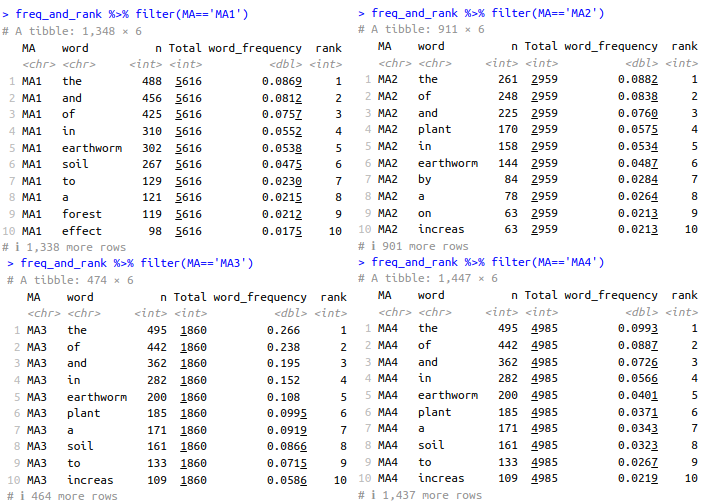
\includegraphics[width=1\textwidth]{word_rank_table.png}
						\caption{Capture d'écran issue de R montrant, pour chaque MA, les mots les plus fréquents rencontrés dans le corpus (rangs décroissants).}\label{Zipf}
						%legende
					\end{center}
				\end{figure}
			\end{column}
		\end{columns}
	\end{frame}

	\begin{frame}
		\frametitle{\underline{Fréquences brutes:}} 
		\begin{columns}
			\begin{column}{0.5\textwidth} % permet diviser la frame en deux colonnes, chacune occupant 50% de l'espace total disponible.
				\begin{enumerate}
					\item Racines les plus fréquentes: \textit{earthworm, soil} et \textit{plant}.
					\item Thème général commun à toutes les MA: \textbf{Rôle écologique du vers de terre.}
				\end{enumerate}
			\end{column}
			\begin{column}{0.5\textwidth}
				\begin{figure}[htb] %le h entre crochet signifie je veux la figure à cet emplacement
					\begin{center} %centrer la figure
						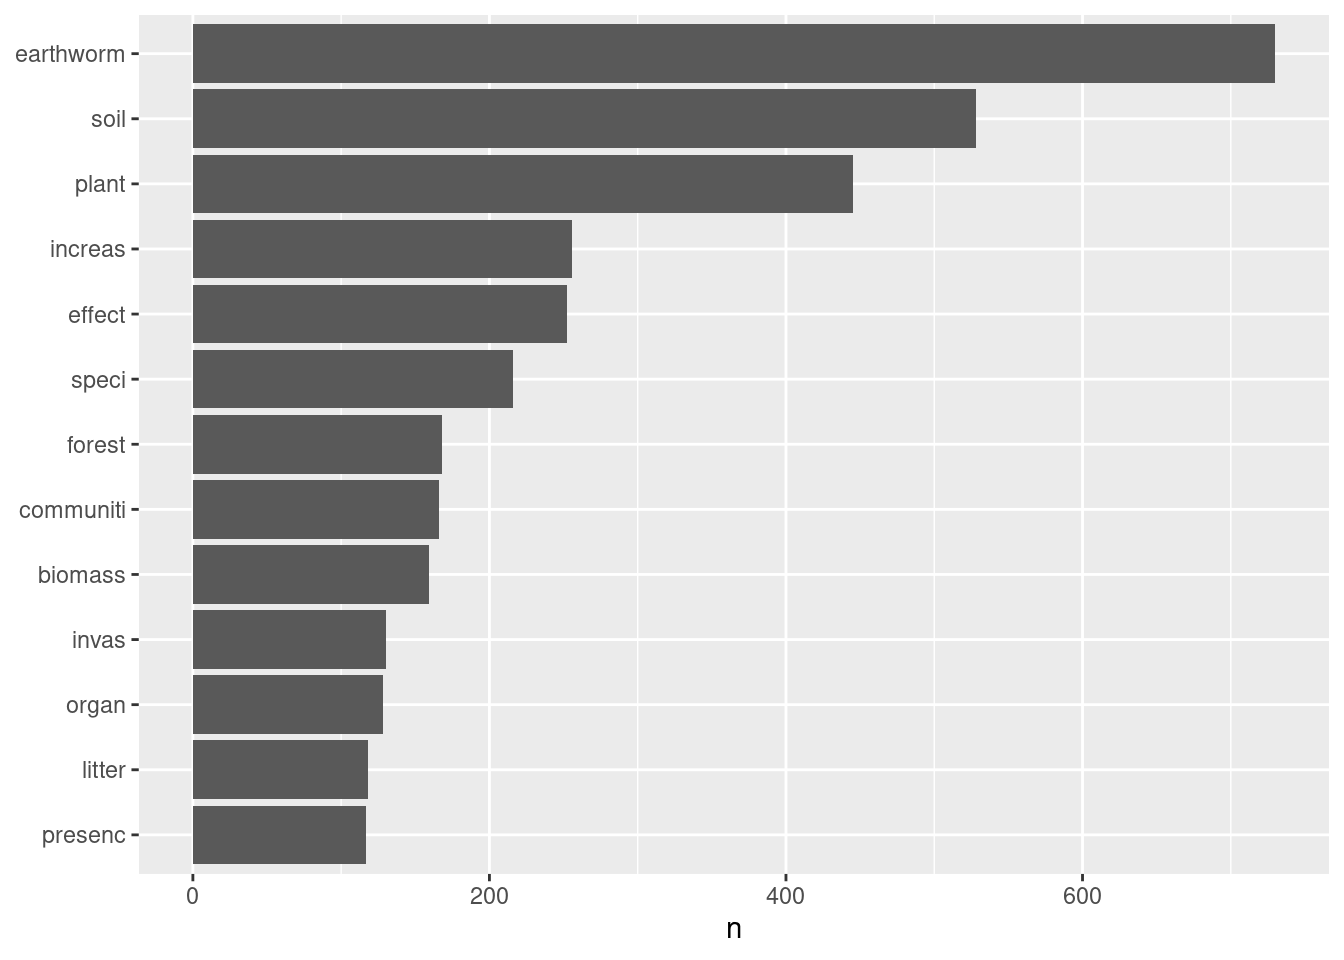
\includegraphics[width=1\textwidth]{freq_all_MA.png}
						\caption{Diagramme à barre représentant les mots les plus fréquents dans l'ensemble des corpus étudiés. Les trois racines les plus fréquentes sont \textit{earthworm, soil} et \textit{plant}.}\label{all_freq}
						%legende
					\end{center}
				\end{figure}
			\end{column}
		\end{columns}
	\end{frame}

	\begin{frame}
		\frametitle{\underline{Comparaison de fréquences:}}
		\begin{columns}
			\begin{column}{0.4\textwidth} % permet diviser la frame en deux colonnes, chacune occupant 50% de l'espace total disponible.
				\begin{enumerate}
					\item "earthworm"= très fréquent dans les 4 MA.
					\item "soil" = très fréquent pour MA1, 2 et 3.
					\item "plant", "community" et "growth" = $\text{MA2} > \text{MA1}$.
					\item "disturb", "density", "plant" = $\text{MA3} > \text{MA1}$.
					\item "forest", "invasive", "exotic" = $\text{MA1} > \text{MA4}$.
					\item "plant", "growth", "fertil" = $\text{MA4} > \text{MA1}$.
				\end{enumerate}
			\end{column}
			\begin{column}{0.6\textwidth}
				\begin{figure}[htb] %le h entre crochet signifie je veux la figure à cet emplacement
					\begin{center} %centrer la figure
						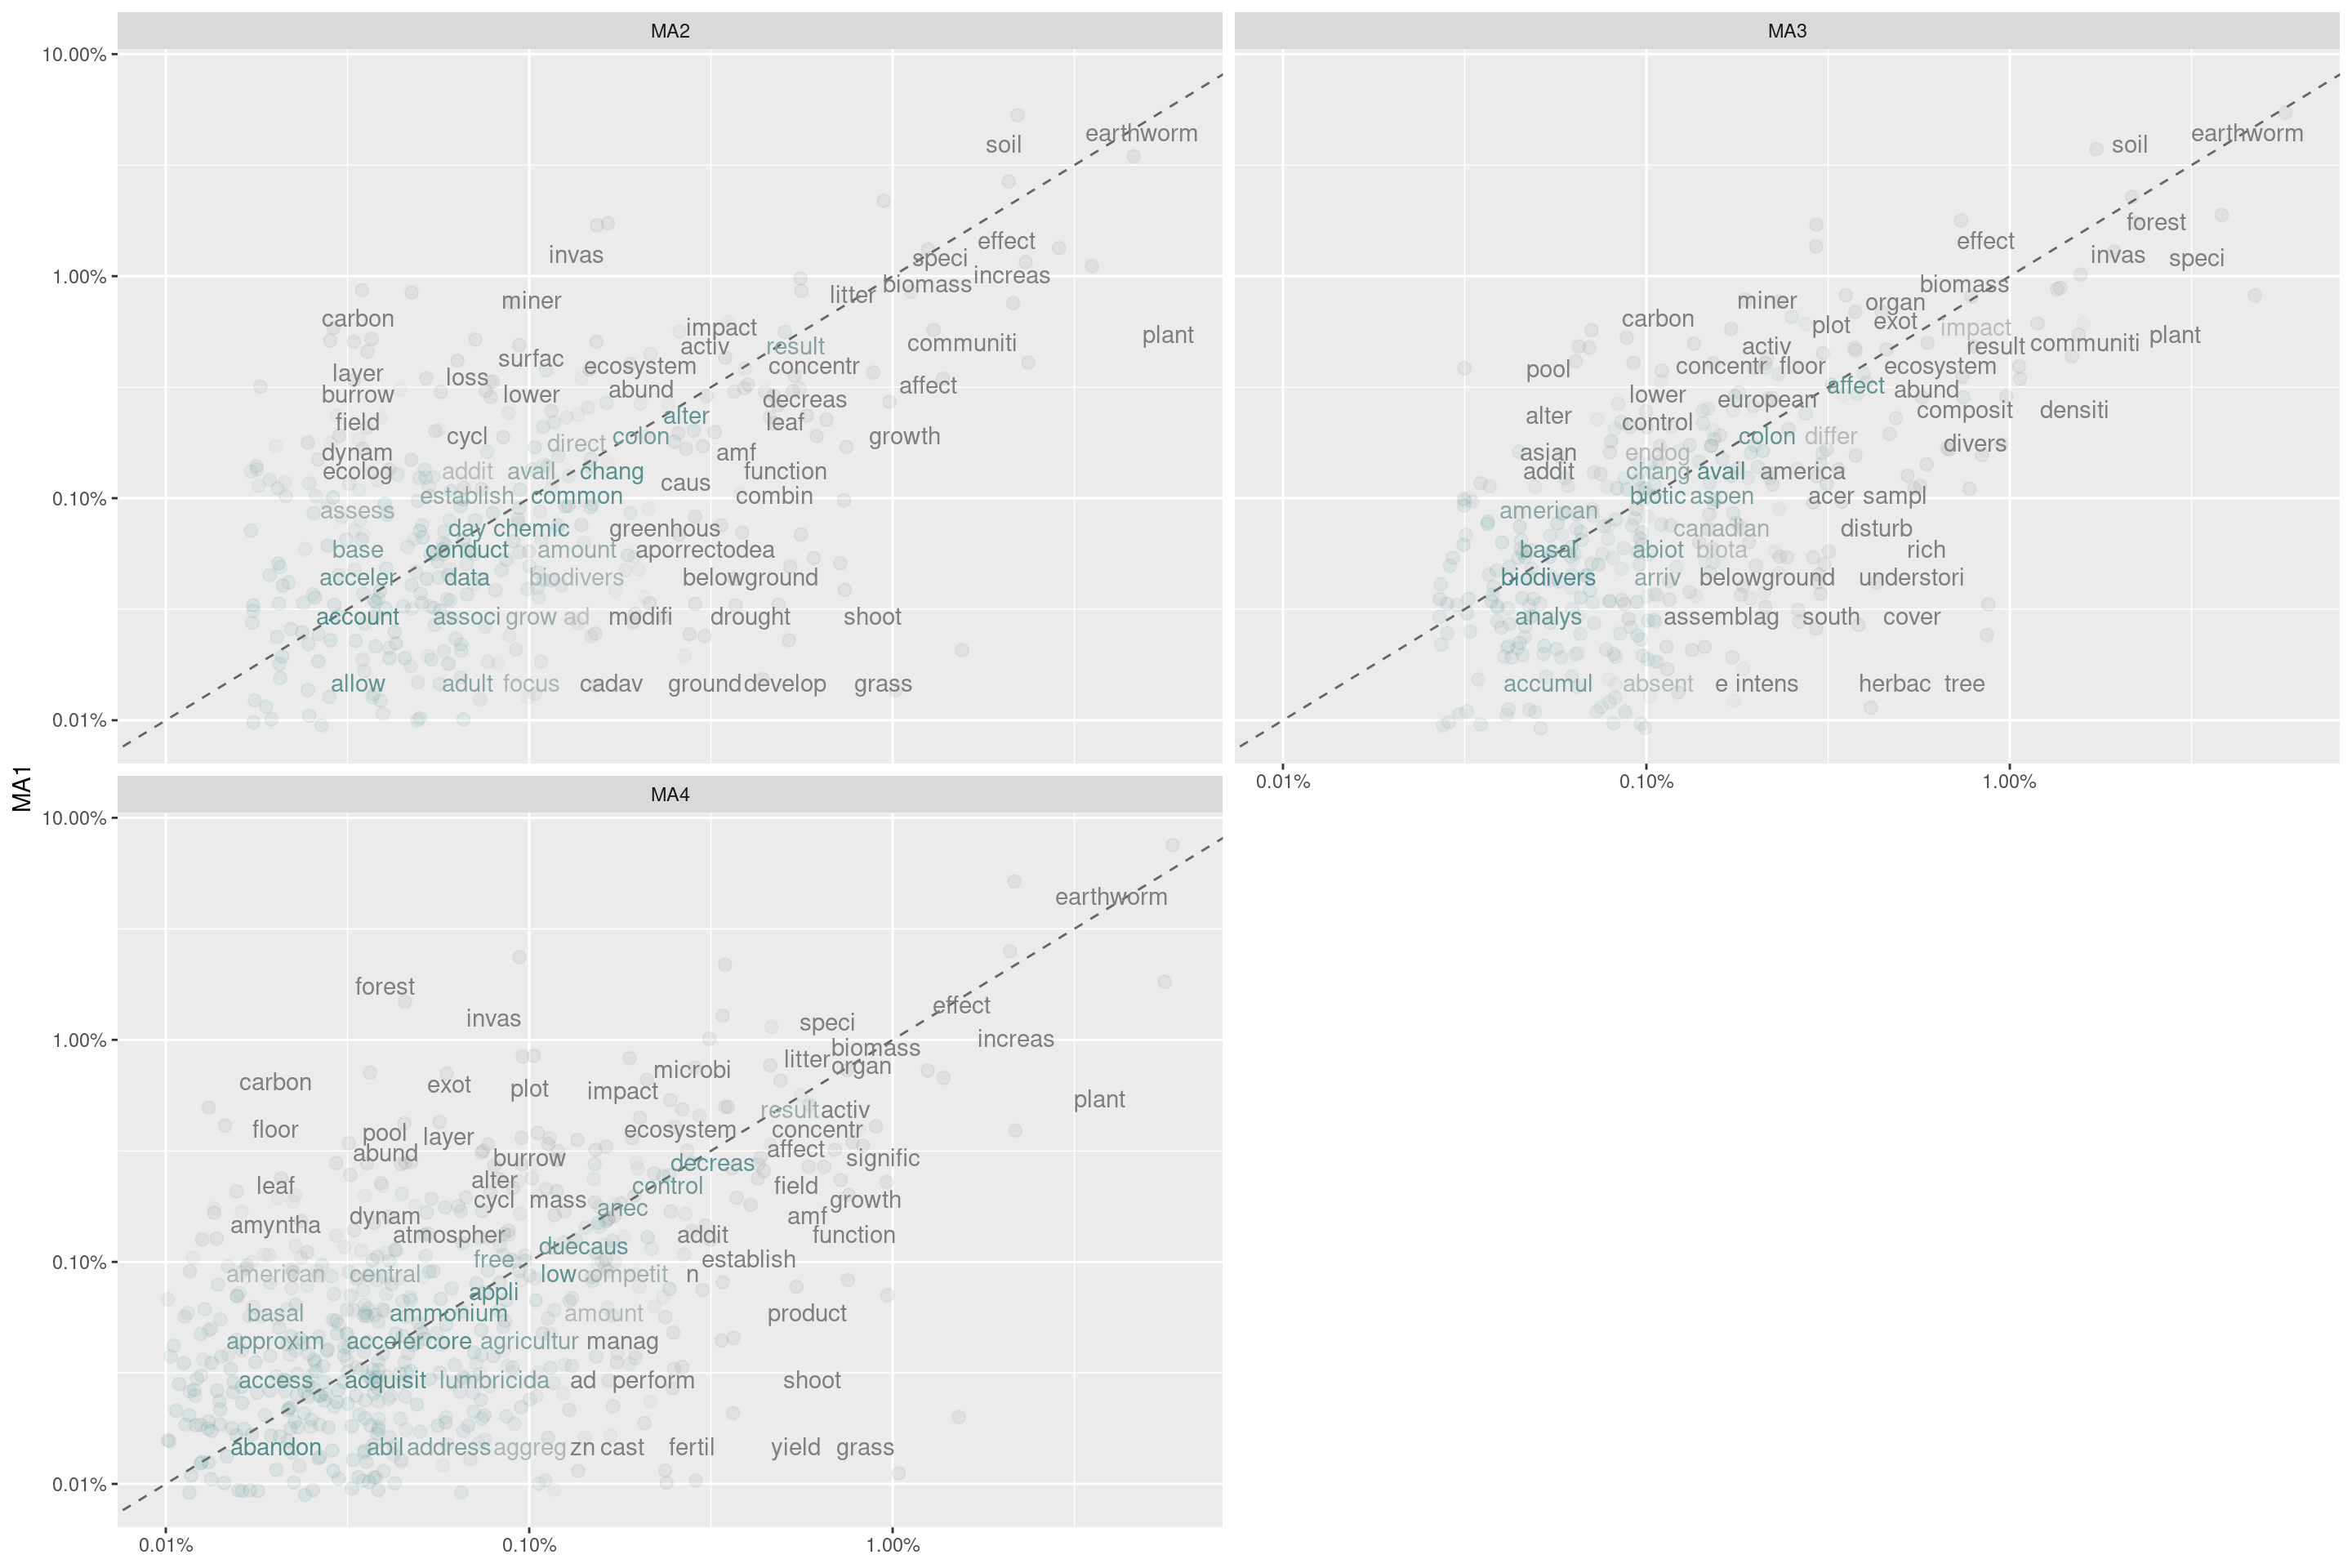
\includegraphics[width=1\textwidth]{scales_graph.png}
						\caption{Log-log scatter plot montrant les corrélations du choix des mots entre la MA1 et les 3 autres MA.}\label{log_log_sp}
						%legende
					\end{center}
				\end{figure}
			\end{column}
		\end{columns}
		\vspace{\baselineskip}
		Here is some rambling text
	\end{frame}

	\begin{frame}
		\frametitle{\underline{Approche TF-IDF (Term frequency x Inverse document frequency):}} 
		\begin{columns}
			\begin{column}{0.5\textwidth} % permet diviser la frame en deux colonnes, chacune occupant 50% de l'espace total disponible.
				\begin{enumerate}
					\item Thèmes majeurs MA1: "earthworm", "soil" et "forest".
					\item Thèmes majeurs MA2: "aphid", "nematod" et "herbivor".
					\item Thèmes majeurs MA3: "eastern", "canopy", "arthropod".
					\item Thèmes majeurs MA4: "grain", "pb", "cu".
				\end{enumerate}
			\end{column}
			\begin{column}{0.5\textwidth}
				\begin{figure}[htb] %le h entre crochet signifie je veux la figure à cet emplacement
					\begin{center} %centrer la figure
						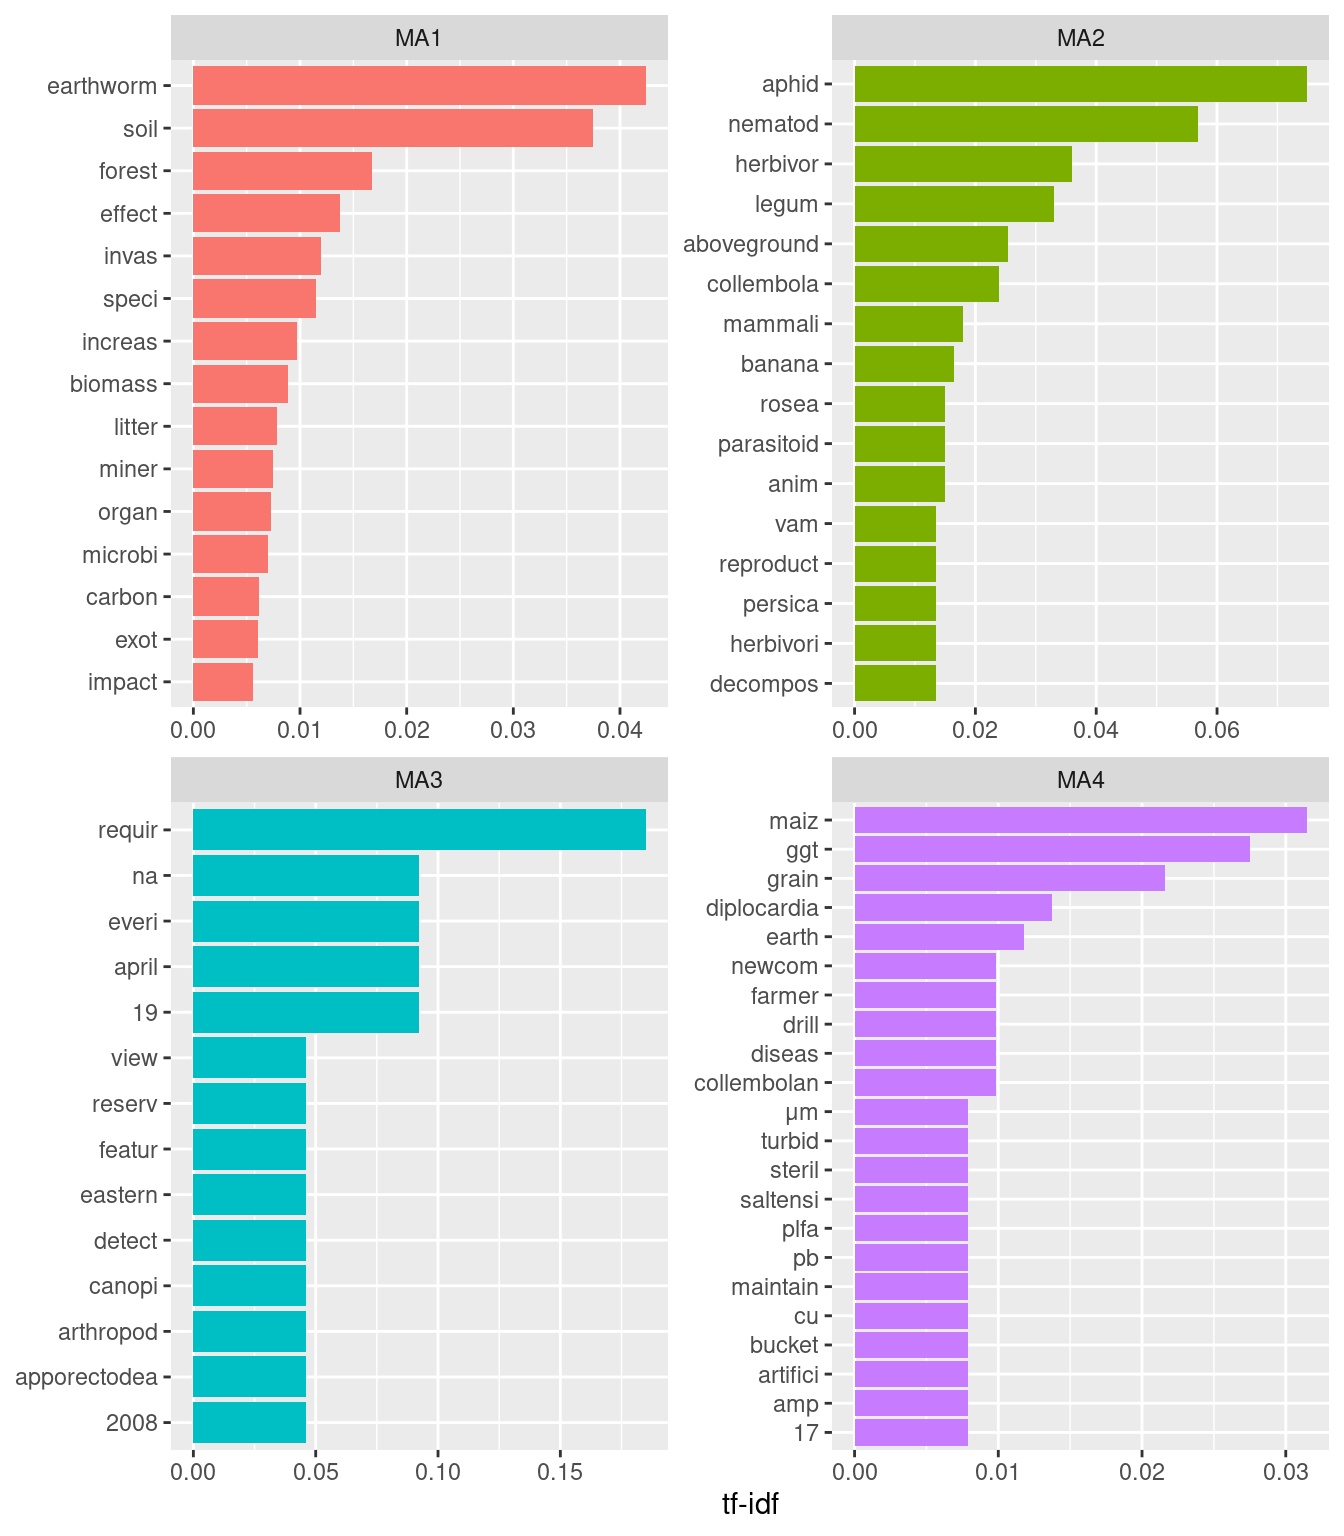
\includegraphics[width=0.7\textwidth]{graphe_tf_idf.png}
						\caption{Ce graphe de tf-idf montre les mots thématiques plus fréquents dans une MA précise que dans l'ensemble du corpus.}\label{tf_idf}
						%legende
					\end{center}
				\end{figure}
			\end{column}
		\end{columns}
	\end{frame}

	\section*{Analyse de bigrammes}
	\subsection*{TF-IDF sur les bigrammes / Réseaux de bigrammes}

	\begin{frame}
		\frametitle{\underline{TF-IDF sur les bigrammes:}} 
		\begin{columns}
			\begin{column}{0.5\textwidth} % permet diviser la frame en deux colonnes, chacune occupant 50% de l'espace total disponible.
				\begin{enumerate}
					\item Thèmes majeurs MA1: "mineral soil",
					"earthworm invasion", "exotic earthworms".
					\item Thèmes majeurs MA2: "soil organisms", "plant responses", "plant mediated".
					\item Thèmes majeurs MA3: "species richness", "earthworm invasion", "native earthworm".
					\item Thèmes majeurs MA4: "soil organisms", "dry weight", "soil fertility".
				\end{enumerate}
			\end{column}
			\begin{column}{0.5\textwidth}
				\begin{figure}[htb] %le h entre crochet signifie je veux la figure à cet emplacement
					\begin{center} %centrer la figure
						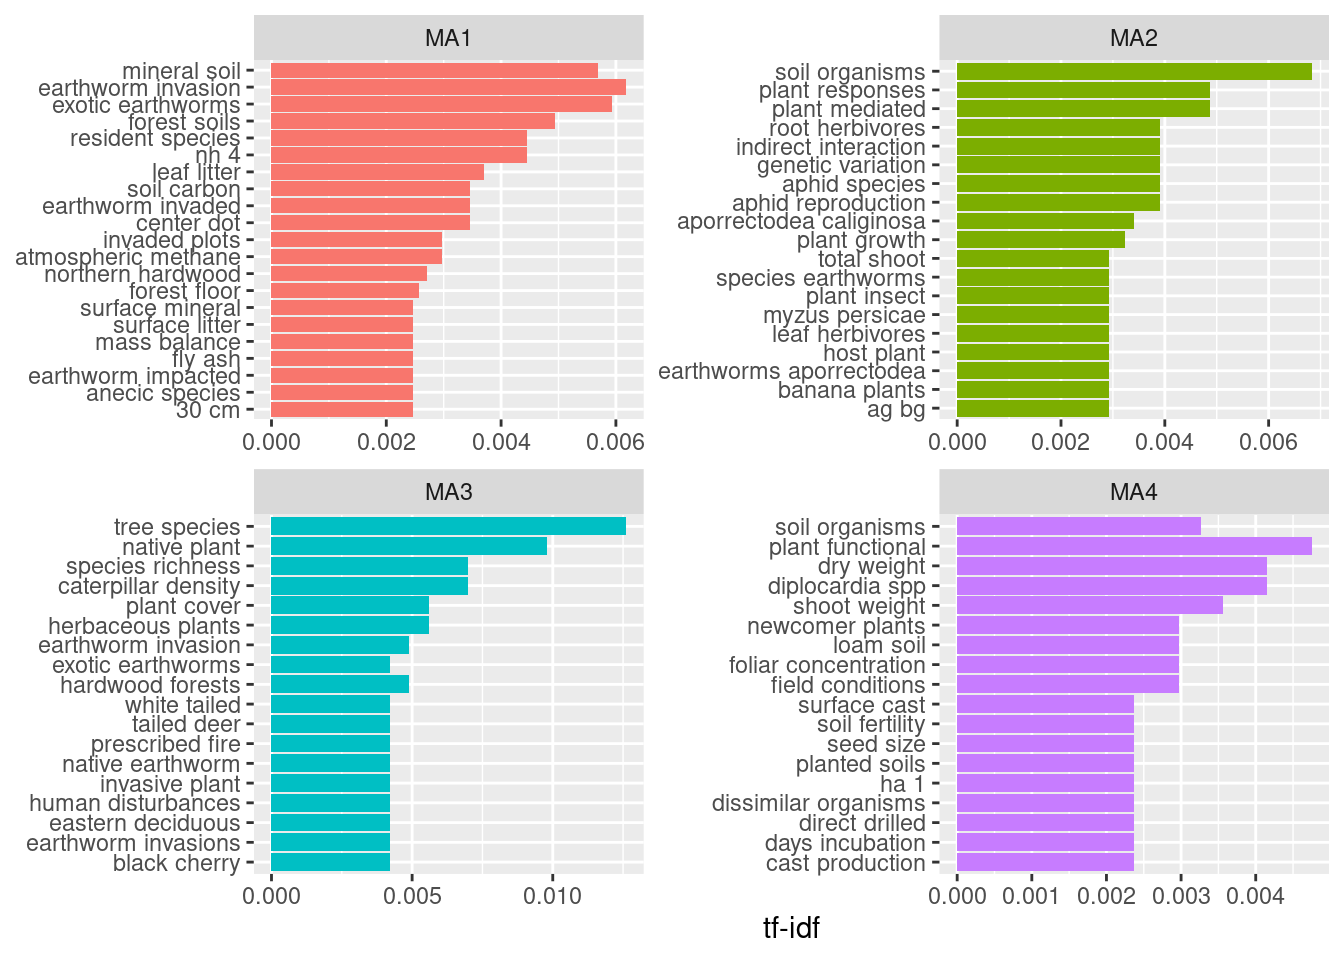
\includegraphics[width=1\textwidth]{bigrammes_tf_idf.png}
						\caption{Ce graphe de tf-idf montre les bigrammes thématiques plus fréquents dans une MA précise que dans l'ensemble du corpus.}\label{bi_tf_idf}
						%legende
					\end{center}
				\end{figure}
			\end{column}
		\end{columns}
	\end{frame}

	\begin{frame}
		\frametitle{\underline{Réseaux de bigrammes:}}
		\begin{columns}
			\begin{column}{0.5\textwidth} % permet diviser la frame en deux colonnes, chacune occupant 50% de l'espace total disponible.
				\begin{enumerate}
					\item Trois centres majeurs: \textbf{"plant", "soil"} et \textbf{"earthworm"}.
					\item Plant: \textit{“plant community”, “plant growth”, “plant communities”}.
					\item Soil: \textit{“mineral soil”, “soil microbial” / “microbial biomass” (forte
					association), “soil organisms”}.
					\item Earthworm: \textit{“earthworm invasion”, “earthworm species”, “earthworm activity”}.
				\end{enumerate}
			\end{column}
			\begin{column}{0.5\textwidth}
				\begin{figure}[htb] %le h entre crochet signifie je veux la figure à cet emplacement
					\begin{center} %centrer la figure
						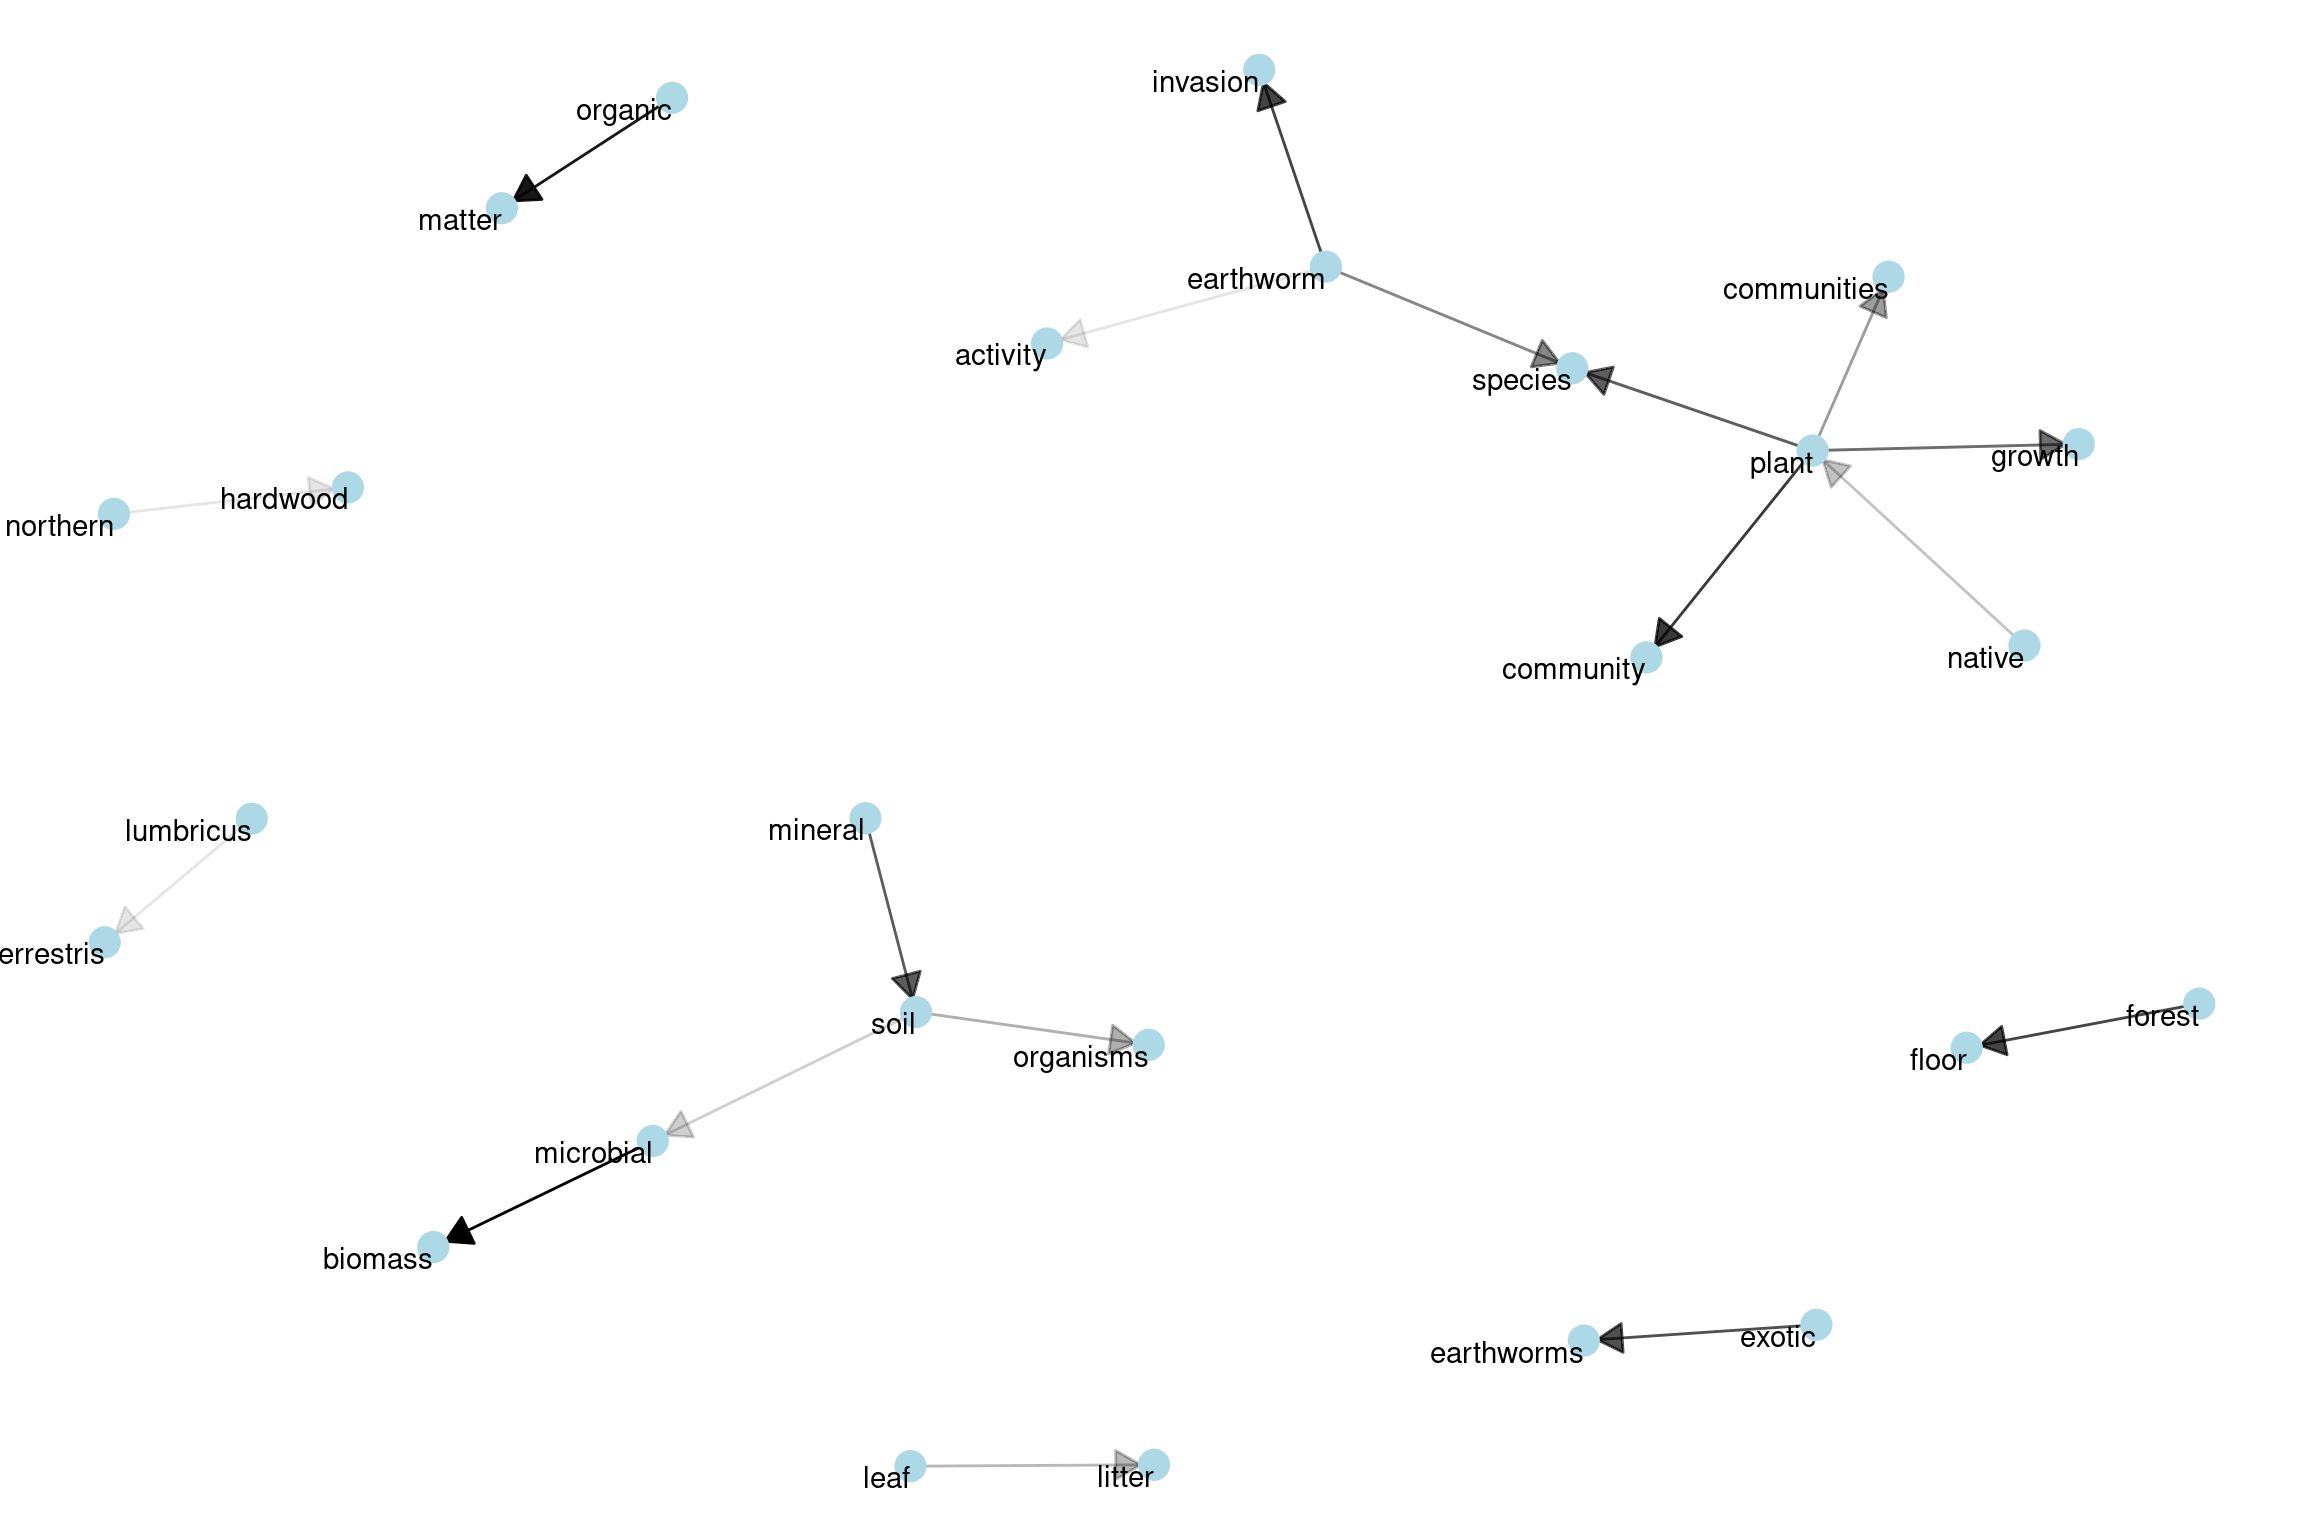
\includegraphics[width=1\textwidth]{network_all_(oriented).png}
						\caption{Réseau de bigrammes orienté montrant les différentes connections (flèches) existant entre les mots (noeuds) de l'ensemble du corpus.}\label{nw_all_oriented}
						%legende
					\end{center}
				\end{figure}
			\end{column}
		\end{columns}
	\end{frame}

	\section*{Analyse de sentiment}
	\subsection*{\textit{Wordcloud} / Contribution / Influence du mot "not" en n-1}

	\begin{frame}
		\frametitle{\textit{\underline{Wordcloud:}}}
		\begin{columns}
			\begin{column}{0.5\textwidth} % permet diviser la frame en deux colonnes, chacune occupant 50% de l'espace total disponible.
				\begin{enumerate}
					\item Principaux contributeurs négatifs (-1 au score de sentiment): \textit{"invasiv", "invad", "loss", "negat"}.
					\item Principaux contributeurs positifs (+1 au score de sentiment): \textit{"effect", "affect", "enhance", "product"}.
				\end{enumerate}
			\end{column}
			\begin{column}{0.5\textwidth}
				\begin{figure}[htb] %le h entre crochet signifie je veux la figure à cet emplacement
					\begin{center} %centrer la figure
						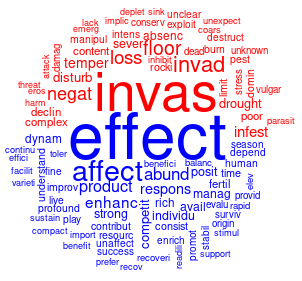
\includegraphics[width=0.7\textwidth]{senti_cloud_all.png}
						\caption{Nuage de mots réalisé sur les données des 4 MA confondues. \textbf{Sentiment négatif: Rouge. Sentiment positif: Bleu.}}\label{senti_wc}
						%legende
					\end{center}
				\end{figure}
			\end{column}
		\end{columns}
	\end{frame}

	\begin{frame}
		\frametitle{\underline{Contribution:}}
		\begin{columns}
			\begin{column}{0.5\textwidth} % permet diviser la frame en deux colonnes, chacune occupant 50% de l'espace total disponible.
				\begin{enumerate}
					\item MA1 et 3: Globalement négatives (\textit{Figure 11, 1. et 3.}) \\
					\textbf{Principaux contributeurs:} "invas", "invad", "loss" (MA1) / "invas, "disturb", "burn" (MA3). 
					\item MA2 et 4: Globalement positives (\textit{Figure 11, 2. et 4.}) \\
					\textbf{Principaux contributeurs:} "enhanc", "strong", "competitiv" (MA1) / "fertil", "enhanc", "competitiv" (MA3).
				\end{enumerate}
			\end{column}
			\begin{column}{0.5\textwidth}
				\begin{figure}[htb] %le h entre crochet signifie je veux la figure à cet emplacement
					\begin{center} %centrer la figure
						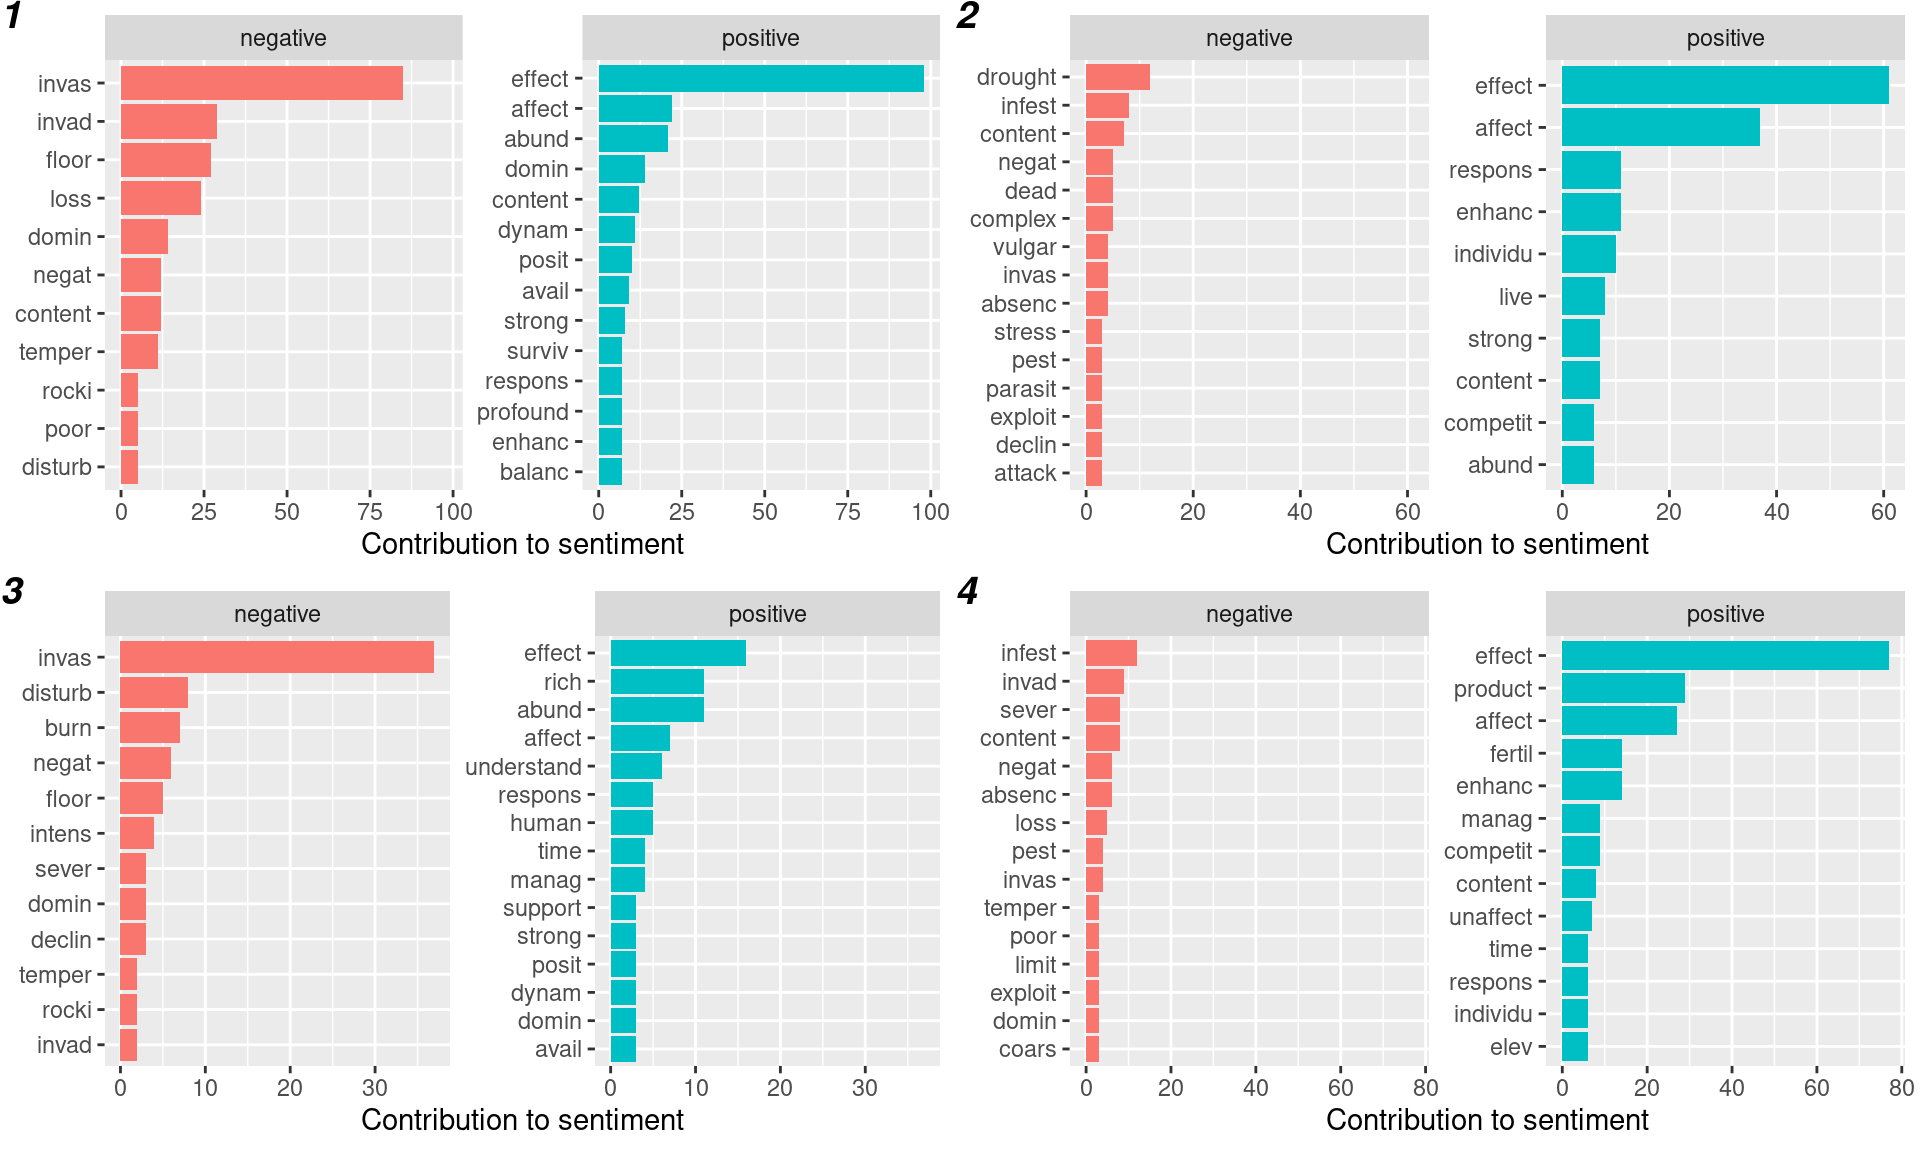
\includegraphics[width=1\textwidth]{senti_contri_each.png}
						\caption{Diagramme à barres présentant, pour chacune des MA, les principaux contributeurs au score de sentiment global. \textbf{Sentiment négatif: Rouge. Sentiment positif: Bleu.}}\label{contri_graph}
						%legende
					\end{center}
				\end{figure}
			\end{column}
		\end{columns}
	\end{frame}

	\begin{frame}
		\frametitle{\underline{Influence du mot "not" en n-1:}}
		\begin{columns}
			\begin{column}{0.6\textwidth} % permet diviser la frame en deux colonnes, chacune occupant 50% de l'espace total disponible.
				\begin{enumerate}
					\item MA1: "benefit", "increase" = positif / "\textbf{not} benefit", "\textbf{not} increase" = négatif.
					\item MA2 / 3: "affected" = négatif / "\textbf{not} affected" = positif.
					\item MA4: "affected" = négatif / "\textbf{not} affected" = positif.
					\item MA4: "responsible" / "\textbf{not} responsible" = Contexte dépendant.
				\end{enumerate}
			\end{column}
			\begin{column}{0.4\textwidth}
					\begin{figure}[htb] %le h entre crochet signifie je veux la figure à cet emplacement
						\begin{center} %centrer la figure
							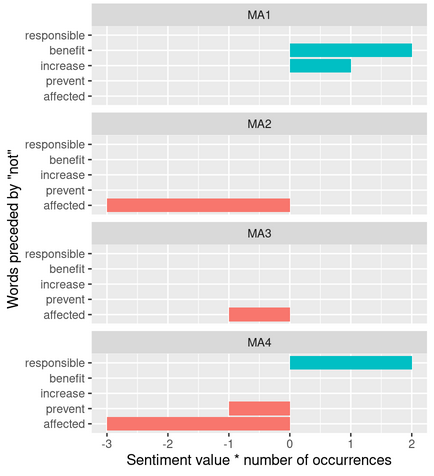
\includegraphics[width=0.8\textwidth]{influence_not_score_senti.png}
							\caption{Diagramme à barres présentant, pour chacune des MA, les erreurs d'attribution de score de sentiment dûes à la présence du mot "not" en n-1.}\label{not}
							%legende
						\end{center}
					\end{figure}
			\end{column}
		\end{columns}
	\end{frame}

	\section*{Conclusion}
	\subsection*{Démarche et résultats, limites}

	\begin{frame}
		\begin{columns}
			\begin{column}{0.5\textwidth} % permet diviser la frame en deux colonnes, chacune occupant 50% de l'espace total disponible.
				\begin{itemize}
					\item Collecte de données textuelles: \textit{Web-scraping} avec Python.
					\item Analyse statistique: \textit{Text-mining} avec R.
					\item MA1 et 3 globalement négatives.
					\item MA2 et 4 globalement positives.
				\end{itemize}
			\end{column}

			\begin{column}{0.5\textwidth}
				\begin{itemize}
					\item Pays d'origine des auteurs non trouvé (non inclus dans la base de données.)
					\item Difficulté à récupérer les abstracts par \textit{Web-scraping}. Complétion manuelle des données.
					\item Approche de \textit{topic modeling} prévue initialement, mais non abordée.
				\end{itemize}
			\end{column}
		\end{columns}
	\end{frame}
\end{document}

















% 15 DIAPOS EN M1 BIMS.

% MANUEL:

% FAIRE UNE FRAME COUPÉE EN 2 AU MILIEU:
%  	\begin{frame}
% 	Bla bla 
% 	\begin{columns}
% 		\begin{column}{0.5\textwidth} % permet diviser la frame en deux colonnes, chacune occupant 50% de l'espace total disponible.
% 			\begin{enumerate}
% 				\item List item 1
% 				\item List item 2
% 			\end{enumerate}
% 		\end{column}
% 		\begin{column}{0.5\textwidth}
% 			\begin{itemize}
% 				\item List item 1
% 				\item List item 2
% 			\end{itemize}
% 		\end{column}
% 	\end{columns}
% 	\vspace{\baselineskip}
	
% 	Here is some rambling text

% \end{frame}

% CAPTION:
% Ne supporte pas le retour à la ligne "\\".